\documentclass[a4paper, 11pt]{article}
\usepackage[margin=1in]{geometry}
\usepackage{preamble}

\title{ELEC4620 Assignment 1}
\author{Deren Teo}

\begin{document}

\maketitle

\section*{Question 1}
\fakesection{1}

The function for a rectangular pulse around $t=0$, with amplitude $A$ and width
$T$, is:
\begin{align*}
    h(t) = \begin{cases}
        A, & |t| < T/2 \\
        0, & |t| > T/2
    \end{cases}
\end{align*}
This is equivalently two step functions of equal magnitude and opposite sign at
$t=\pm T/2$. Hence, the derivative of the rectangular pulse is composed of two
impulses of equal magnitude and opposite sign, coinciding in time with the
discontinuities in the pulse.
\begin{align*}
    h'(t) = A \delta(t+\frac{T}{2}) - A \delta(t-\frac{T}{2})
\end{align*}
Taking the Fourier transform of the derivative, which by definition is
\begin{align*}
    \widehat{H'}(f) \coloneqq \int_{-\infty}^{\infty} h'(t) e^{-j2\pi ft} dt
\end{align*}
we aim to evaluate the following expression, split into two integrals for
simplicity.
\begin{align*}
    \widehat{H'}(f) = A \int_{-\infty}^{\infty} \delta(t + \frac{T}{2}) e^{-j2\pi ft} dt -
            A \int_{-\infty}^{\infty} \delta(t - \frac{T}{2}) e^{-j2\pi ft} dt
\end{align*}
By definition of the Dirac delta, $\delta(t-T)$, for arbitrary $T$:
\begin{align*}
    \delta(t-T) = \begin{cases}
        \infty, & t = T \\
        0,      & t \neq T
    \end{cases}
    && \text{and} &&
    \int_{-\infty}^{\infty} \delta(t-T) dt = 1
\end{align*}
Therefore, the Fourier transform of the derivative simplifies to
\begin{align*}
    \widehat{H'}(f) = Ae^{-j2\pi f(-T/2)} - Ae^{-j2\pi f(T/2)}
          = A \left[ e^{j\pi fT} - e^{-j\pi fT}\right]
\end{align*}
Finally, we can integrate in the time domain by dividing by $j2\pi f$ in the
frequency domain.
\begin{align*}
    H(f) = \frac{A}{j2\pi f} \left[ e^{j\pi fT} - e^{-j\pi fT}\right]
\end{align*}
Some re-arranging and substitutions can be performed to neaten the result, if desired:
\begin{align*}
    H(f) = \frac{A}{\pi f}\sin(\pi Tf)
         = AT\frac{\sin(\pi Tf)}{\pi Tf}
         = AT\text{sinc}(Tf)
\end{align*}
Thus, we have derived the Fourier transform of a rectangular pulse.

\newpage

We now repeat this procedure for a triangle function using a double derivative.
The function for a triangular pulse around $t=0$, with amplitude $A$ and width $T$, is:
\begin{align*}
    h(t) = \begin{cases}
        A(1 - 2|t|/T), & |t| \leq T/2 \\
        0,             & |t| > T/2
    \end{cases}
\end{align*}
The first derivative produces a result composed of two rectangular pulses of
equal magnitude and opposite sign, or equivalently three step functions.
\begin{align*}
    h'(t) = \begin{cases}
        2A/T, & -T/2 \leq t \leq 0 \\
       -2A/T, &  0 \leq t \leq T/2 \\
        0,    & |t| > T/2
    \end{cases}
\end{align*}
Hence, as before, the second derivative is composed of three impulses coinciding
with the discontinuities in the first derivative.
\begin{align*}
    h''(t) = \frac{2A}{T}\delta(t+\frac{T}{2}) -
             \frac{4A}{T}\delta(t) +
             \frac{2A}{T}\delta(t-\frac{T}{2})
\end{align*}
The Fourier transform of the second derivative is therefore
\begin{align*}
    \widehat{H''}(f) = \frac{2A}{T}\int_{-\infty}^\infty \delta(t+\frac{T}{2}) e^{-j2\pi ft} dt -
             \frac{4A}{T}\int_{-\infty}^\infty \delta(t) e^{-j2\pi ft} dt +
             \frac{2A}{T}\int_{-\infty}^\infty \delta(t-\frac{T}{2}) e^{-j2\pi ft} dt
\end{align*}
Once again, using the definition of the Dirac delta, the Fourier transform
simplifies to
\begin{align*}
    \widehat{H''}(f) = \frac{2A}{T} \left[ e^{-j2\pi f(-T/2)} - 2e^{-j2\pi f(0)} + e^{-j2\pi f(T/2)} \right]
\end{align*}
and further to
\begin{align*}
    \widehat{H''}(f) = \frac{2A}{T} \left[ e^{j\pi fT} - 2 + e^{-j\pi fT} \right]
\end{align*}
We can integrate twice in the time domain by dividing by $(j2\pi f)^2$ in the frequency
domain.
\begin{align*}
    H(f) = \frac{2A}{(j2\pi f)^2 T} \left[ e^{j\pi fT} - 2 + e^{-j\pi fT} \right]
         = \frac{-A}{2\pi^2f^2 T} \left[ e^{j\pi fT} - 2 + e^{-j\pi fT} \right]
\end{align*}
Finally, as with the rectangular pulse, we can re-arrange this result into a
more familiar form:
\begin{align*}
    H(f) = \frac{A}{\pi^2f^2T}(1 - \cos(\pi Tf))
\end{align*}
Thus, we have derived the Fourier transform of a triangular pulse.

Having derived the Fourier transforms of the two functions, we are interested in
comparing the rates at which their magnitudes decrease as frequency increases.
We note the only term contributing to a change in magnitude with frequency is
the $1/f$ term for the rectangular pulse, and the $1/f^2$ term for the
triangular pulse.

Indeed, in general, if a function has discontinuities in the $n^\text{th}$
derivative, the sidelobes of its Fourier transform will fall off as $1/f^{n+1}$.
Intuitively, this is because the function must be derived $n+1$ times to obtain
a number of impulses which can be Fourier transformed without yielding any
frequency-dependent coefficients. The transform of the derivative is then
integrated $n+1$ times by dividing by $(j2\pi f)^{n+1}$; hence, the term
$1/f^{n+1}$ is produced.

\newpage

Figure \ref{fig:q1_sidelobes} presents the Fourier transforms of the rectangular
and triangular pulses, enabling a visual comparison of the rates at which their
sidelobes fall off.

\begin{figure}[ht]
    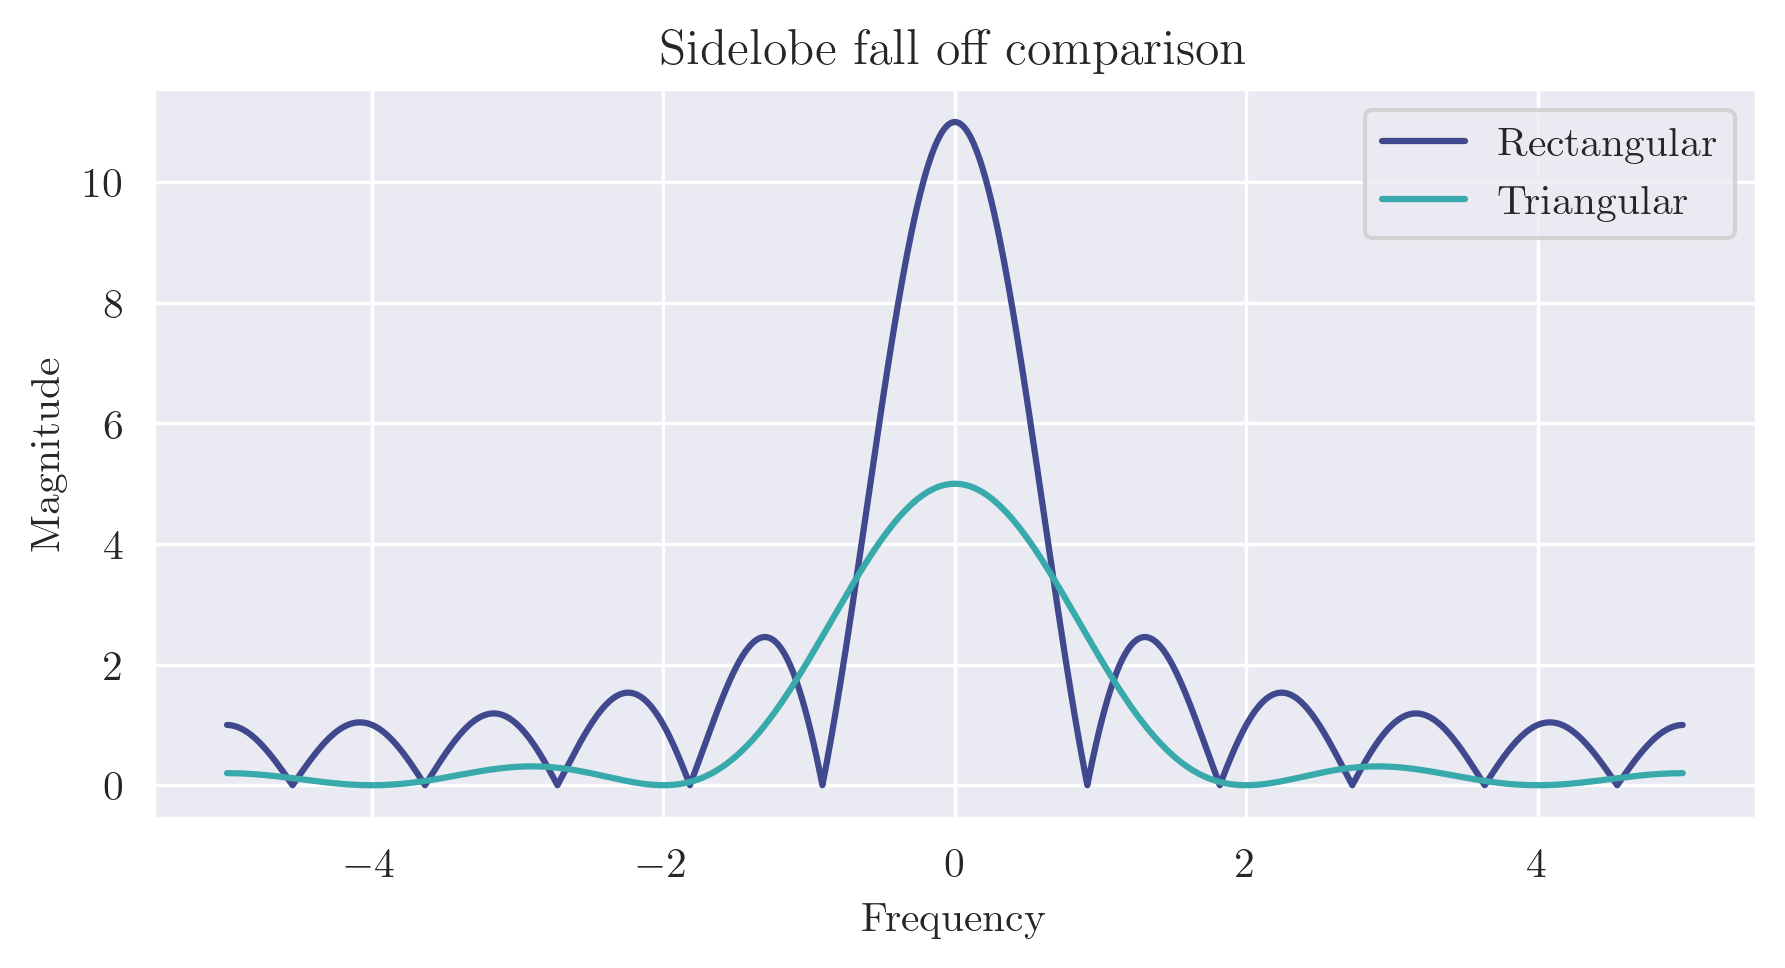
\includegraphics[width=0.95\textwidth]{images/q1_sidelobes.png}
    \caption{Fourier transform sidelobe fall off comparison: rectangular and
             triangular pulses.}
    \label{fig:q1_sidelobes}
\end{figure}

\newpage
\section*{Question 2}
\fakesection{2}

Denote the given polynomials in $z$ by $X(z)$ and $Y(z)$, as follows:
\begin{align*}
    X(z) &= 1 + 2z^{-1} + 6z^{-2} + 11z^{-3} + 15z^{-4} + 12z^{-5} \\
    Y(z) &= 1 - 3z^{-1} - 3z^{-2} + 7z^{-3} - 7z^{-4} + 3z^{-5}
\end{align*}
Their corresponding vectors are constructed from their respective coefficients:
\begin{align*}
    v_X = [1, 2, 6, 11, 15, 12] && \text{and} && v_Y = [1, -3, -3, 7, -7, 3]
\end{align*}
The result of multiplying $X(z)$ and $Y(z)$ can be obtained by convolving their
respective vectors and interpreting the outcome as the coefficients of the
polynomial product. That is,
\begin{align*}
    v_X \ast v_Y = [1, -1, -3, -6, -29, -35, -40, 10, 12, -39, 36]
\end{align*}
This can be calculated using the \texttt{convolve} function from the Python
\texttt{scipy.signal} library:
\begin{center}
    \texttt{signal.convolve(vx, vy, mode="full", method="direct")}
\end{center}
which calculates the full discrete linear convolution, automatically
zero-padding the vectors as necessary, using traditional convolution (i.e.
multiplying and summing, as opposed to the FFT).

Hence, we can interpret the convolution result as the polynomial product of
$X(z)$ and $Y(z)$ as
\begin{align*}
    1 - z^{-1} - 3z^{-2} - 6z^{-3} - 29z^{-4} - 35z^{-5} - 40z^{-6} + 10z^{-7} +
    12z^{-8} - 39z^{-9} + 36z^{-10}
\end{align*}
Since convolution is equivalent to multiplication in the Fourier domain, we
could equivalently Fourier transform both vectors, multiply in the Fourier
domain, then perform an inverse Fourier transform to obtain the same vector of
coefficients derived above.

When doing this in Python, we must manually zero-pad the vectors before
performing the FFT.
\begin{center}
    \texttt{vx = np.pad(vx, (0, len(vy) - 1))} \\
    \texttt{vy = np.pad(vy, (0, len(vx) - 1))}
\end{center}
Here, the Python \texttt{numpy} package is used to zero-pad both vectors on the
right side only to the appropriate length. Then, \texttt{fft} and \texttt{ifft}
from \texttt{scipy.fft} can be applied:
\begin{center}
    \texttt{ifft(fft(vx) * fft(vy))}
\end{center}
This calculates the following vector, which we can observe is identical to the
vector determined through direct convolution:
\begin{center}
    \texttt{[  1.  -1.  -3.  -6. -29. -35. -40.  10.  12. -39.  36.]}
\end{center}
Hence, the same polynomial product can be constructed from either convolving the
vector representations of the polynomials, or multiplying the Fourier transforms
of the vectors, then taking the inverse Fourier transform.

\newpage
\section*{Question 3}
\fakesection{3}

Given the following numbers in base 10, we seek to apply similar methods to
Question 2 to multiply the numbers, first using convolution, then using Fourier
transform techniques.
\begin{align*}
    x = 8755790 && \text{and} && y = 1367267
\end{align*}
First, however, we can perform regular multiplication to determine the correct
answer that we should get from the convolution and Fourier transform methods:
\begin{align*}
    8755790 \times 1367267 = 11971502725930
\end{align*}
Next, the numbers are constructed digit-wise into vectors:
\begin{align*}
    v_x = [8, 7, 5, 5, 7, 9, 0] && \text{and} && v_y = [1, 3, 6, 7, 2, 6, 7]
\end{align*}
As before, the result of multiplying $x$ and $y$ can be obtained by convolving
their respective vectors. However, the ``carry" step must then be performed to
produce a number in base 10.

Once again, using \texttt{convolve} from \texttt{scipy.signal} with the same
keyword arguments:
\begin{align*}
    v_x \ast v_y = [8, 31, 74, 118, 117, 157, 212, 192, 142, 95, 103, 63, 0]
\end{align*}
Now, however, unlike with the polynomial multiplication, we cannot expect to
arrive at the correct value by simply stringing together all of these digits.
Instead, starting from the right, each value must be taken modulo 10, and the
remainder added to the value immediately to the left. This yields the following
vector, which now can be concatenated into the result of $x \times y$:
\begin{align*}
    [1, 1, 9, 7, 1, 5, 0, 2, 7, 2, 5, 9, 3, 0] \longrightarrow 11971502725930
\end{align*}
Naturally, the same outcome can be achieved by Fourier transforming the vectors,
multiplying in the Fourier domain, then inverse Fourier transforming the result.
Again, in Python, the vectors must be zero-padded before performing the FFT.
\begin{center}
    \texttt{vx = np.pad(vx, (0, len(vy) - 1))} \\
    \texttt{vy = np.pad(vy, (0, len(vx) - 1))}
\end{center}
Then, using the same Python function calls as from Question 2:
\begin{center}
    \texttt{ifft(fft(vx) * fft(vy)) =}
        [8.  31.  74. 118. 117. 157. 212. 192. 142.  95. 103.  63.   0.]
\end{center}
The result is identical to the vector produced by convolution. Therefore,
applying the same ``carrying'' process will yield the same number result.

Hence, integer multiplication also can be accomplished by either convolving the
vector representations of the numbers and converting to base 10, or multiplying
the Fourier transforms of the vectors, then taking the inverse Fourier transform
and converting to base 10.

\newpage
\section*{Question 4}
\fakesection{4}

\begin{enumerate}[label=\alph*)]

    \item First, we individually transform the sequences using the \texttt{fft}
    function from \texttt{scipy.fft}:
    \begin{align*}
        \texttt{fft(x)} = [&34,\ -1.879+j6.536,\ -5+j7,\ -6.121+j0.536,\ \\
                           &0,\ -6.121-j0.536,\ -5-j7,\ -1.879-j6.536] \\
        \texttt{fft(y)} = [&28,\ 2.243+j4.243,\ -2-j2,\ -6.243+j4.243,\ \\
                           &-8,\ -6.243-j4.243,\ -2+j2,\ 2.243-j4.243]
    \end{align*}
    Now, we combine $x$ and $y$ element-wise into a single complex vector:
    \begin{align*}
        z = [1+j\ \ 2+j5\ \ 4+j3\ \ 4+j\ \ 5+j3\ \ 3+j5\ \ 7+j3\ \ 8+j7]
    \end{align*}
    and Fourier transform this to obtain:
    \begin{align*}
        \texttt{fft(z)} = [&34+j28,\ -6.121+j8.778,\ -3+j5,\ -10.364-j5.707,\ \\
                           &-j8,\ -1.879-j6.778,\ -7-j9,\ 2.364-j4.293]
    \end{align*}
    The Fourier transforms of $x$ and $y$ can be determined from the
    Fourier transform of $z$ as
    \begin{align*}
        X &= \Ev(\Re(Z)) + j\Od(\Im(Z)) \\
        Y &= \Ev(\Im(Z)) - j\Od(\Re(Z))
    \end{align*}
    where $Z$ is the Fourier transform of $z$. Since $x$ is purely real and $y$
    purely imaginary, the Fourier transform of $x$ has a purely even real
    component and purely odd imaginary component, and vice versa for the Fourier
    transform of $y$. Even and odd components are orthogonal; hence, $X$ and $Y$
    can be independently reconstructed.

    The even and odd components of a sequence $H(n)$ are determined as:
    \begin{align*}
        \Ev(n) = \frac{H(n)+H(-n)}{2} && \Od(n) = \frac{H(n)-H(-n)}{2}
    \end{align*}
    where $H(-n)$ is the vector $H$ with all elements after the first in
    reversed order. Hence,
    \begin{align*}
        \Ev(\Re(Z)) &= [34,\ -1.879,\ -5,\ -6.121,\ 0,\ -6.121,\ -5,\ -1.879] \\
        \Od(\Im(Z)) &= [0,\ 6.536,\ 7,\ 0.536,\ 0,\ -0.536,\ -7,\ -6.535] \\
        \Ev(\Im(Z)) &= [28,\ 2.243,\ -2,\ -6.243,\ -8,\ -6.243,\ -2,\ 2.243] \\
        \Od(\Re(Z)) &= [0,\ -4,\ 243,\ 2,\ -4,243,\ 0,\ 4.243,\ -2,\ 4.243]
    \end{align*}
    wherein from the second element of each vector onward, the even and odd
    symmetries can be observed. Finally, we can reconstruct the individual
    Fourier transforms of $x$ and $y$:
    \begin{align*}
        X = [&34,\ -1.879+j6.536,\ -5+j7,\ -6.121+j0.536,\ \\
             &0,\ -6.121-j0.536,\ -5-j7,\ -1.879-j6.536] \\
        Y = [&28,\ 2.243+j4.243,\ -2-j2,\ -6.243+j4.243,\ \\
             &-8,\ -6.243-j4.243,\ -2+j2,\ 2.243-j4.243]
    \end{align*}
    Comparing these vectors to those determined individually at the start, we
    can see they are identical. Therefore, we have shown that the double
    transform algorithm gives the same answer as directly transforming the
    sequences.

\newpage

    \item In the previous part, the double transform algorithm was applied to
    sequences of equal length. However, it is also applicable to sequences of
    unequal length by right-padding the shorter sequence with zero. For example,
    \begin{align*}
        x = [1\ 2\ 4\ 4\ 5\ 3\ 7\ 8] && y = [1\ 5\ 3\ 1\ 3\ 5\ 3]
    \end{align*}
    The individual Fourier transforms of $x$ and $y$ are:
    \begin{align*}
        \texttt{fft(x)} = [&34,\ -1.879+j6.536,\ -5+j7,\ -6.121+j0.536 \\
                           &0,\ -6.121-j0.536,\ -5-j7,\ -1.879-j6.536] \\
        \texttt{fft(y)} = [&21,\ 0.604+j1.254,\ -5.494-j4.381,\ -2.110-j0.482 \\
                           &-2.110+j0.482,\ -5.494+j4.381,\ 0.604-j1.254]
    \end{align*}
    As before, we combine $x$ and $y$ element-wise into a single complex vector,
    but this time we must right-pad $y$ with zero such that the vectors are
    equal length.
    \begin{align*}
        z = [1+j\ \ 2+j5\ \ 4+j3\ \ 4+j\ \ 5+j3\ \ 3+j5\ \ 7+j3\ \ 8+j0]
    \end{align*}
    The Fourier transform of $z$ is
    \begin{align*}
        \texttt{fft(z)} = [&34+j21,\ -1.172+j3.828,\ 4+j5,\ -5.414-j0.757,\\
                           &-j,\ -6.828-j1.828,\ -14-j9,\ -2.586-j9.243]
    \end{align*}
    Again, the Fourier transforms of $x$ and $y$ can individually be determined
    from $Z$ using the even and odd components of the real and imaginary parts
    of $Z$, per part (a). Hence,
    \begin{align*}
        \Ev(\Re(Z)) = []
    \end{align*}

\end{enumerate}

\newpage
\section*{Question 5}
\fakesection{5}

\end{document}
